% Load preamble
\documentclass[../main.tex]{subfiles}

\begin{document}
	\subsection{Príklad druhý}
    \subsubsection{Opis systému}
	Majme systém, ktorý je určený stavovým opisom \cref{eqn:svlvs2_rovniceSystemu}. Bloková schéma systému je na \cref{fig:svlvs2_obrazokModelSystemu}.
	\begin{equation}
		\begin{aligned}
		\dot{x_1} &= x_1 + x_2 - x_3 + sin(x_2) 			\\
		\dot{x_2} &= - x_1 - x_2 						\\
		\dot{x_3} &= cos(x_2) (sin(x_2) - x_3) - u 	\\
		y &= x_1
		\end{aligned}
		\label{eqn:svlvs2_rovniceSystemu}
	\end{equation}

	\begin{figure}[h!]
		\centering
		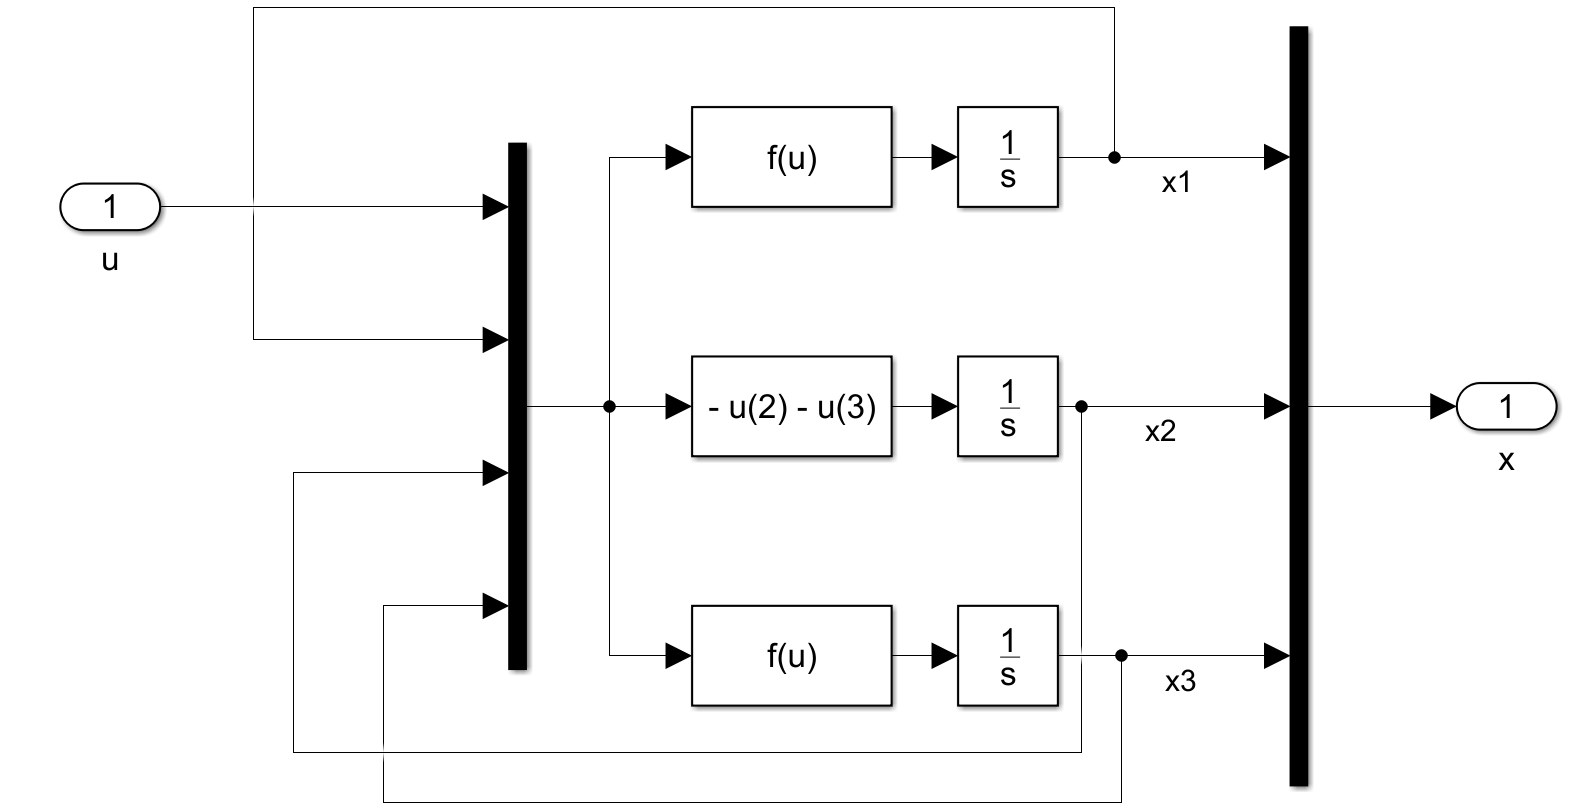
\includegraphics[width=0.8\linewidth]{ModelSystemu}
		\caption{Bloková schéma systému z \cref{eqn:svlvs2_rovniceSystemu}}
		\label{fig:svlvs2_obrazokModelSystemu}
	\end{figure}

    \subsubsection{Rovnovažné stavy}
Tento systém ma stavy $x_1$, $x_2$ a $x_3$. Stav $x_1$ je zároveň výstupom systému.
Bod [0 0 0] je rovnovážny stav systému. V tomto bode sú časové derivácie všetkých stavových premenných rovné nule.

	\begin{equation}
		\begin{aligned}
		\dot{x_1}|_{x_1 = x_2 = x_3 = 0} &= 0 + 0 - 1 + sin(0) = 0 					\\
		\dot{x_2}|_{x_1 = x_2 = x_3 = 0} &= -0 - 0 = 0 							\\
		\dot{x_3}|_{x_1 = x_2 = x_3 = 0} &= cos(0)sin(0) - 0cos(0) - 0 = 0 			\\
		\end{aligned}
		\label{eqn:svlvs2_rovniceRovnovaznyStav}
	\end{equation}

    \subsubsection{Prvý krok - nájdenie transformačných vzťahov}
	Našim cieľom je riadiť tento systém tak, aby výstup $y$ dosiahol žiadanú hodnotu $r$. Systém obsahuje nelinearity v dvoch rovniciach, preto je ťažké určiť zákon riadenia len pohľadom na tieto rovnice. Použijeme metódu Vstupno-stavovej linearizácie, pri ktorej navrhneme linearizačnú slučku, s ktorou sa náš systém bude správať ako lineárny. Pre tento lineárny systém potom navrhneme regulátor, ktorý zabezpečí že sa výstup systému ustáli na žiadanej hodnote.

Prvým krokom metódy je určenie transformačných vzťahov \cref{eqn:svlvs2_transformacneRovnice}.

	\begin{equation}
		\begin{aligned}
		z_1 &= -x_2 													\\
		z_2 &= x_1 + x_2												\\
		z_3 &= sin(x_2) - x_3 											\\
		\end{aligned}
		\label{eqn:svlvs2_transformacneRovnice}
	\end{equation}

    \subsubsection{Druhý krok - transformácia systému}
Druhým krokom je transformácia nášho systému zo stavov $x_1$, $x_2$ a $x_3$ na stavy $z_1$, $z_2$ a $z_3$. To dosiahneme derivovaním transformačných vzťahov (v čase) a dosadením vzťahov z pôvodných rovníc.
	\begin{equation}
        \begin{aligned}
        \dot{z_1} &= -\dot{x_2} \\
                  &= x_1 + x_2 \\
                  &=  z_2 \\
        \end{aligned}
	\end{equation}

	\begin{equation}
        \begin{aligned}
            \dot{z_2} &= \dot{x_1} + \dot{x_2}  \\
                      & = x_1 + x_2 - x_3 + sin(x_2) - x_1 - x_2  \\
                      &= z_3 	\\
        \end{aligned}
	\end{equation}

	\begin{equation}
        \begin{aligned}
            \dot{z_3} &= cos(x_2)\dot{x_2} - \dot{x_3} \\
                      &= cos(x_2)(-x_1 -x_2) -cos(x_2)(sin(x_2) - x_3) + u \\
                      &= u - cos(z_1)(z_2+z_3) 	\\
        \end{aligned}
	\end{equation}
	Transformovaný systém potom opisujú  \cref{eqn:svlvs2_transformovanySystem}.
	\begin{equation}
		\begin{aligned}
		\dot{z_1} &=  z_2												\\
		\dot{z_2} &=  z_3												\\
		\dot{z_3} &=  u - cos(z_1)(z_2+z_3)									\\
		\end{aligned}
		\label{eqn:svlvs2_transformovanySystem}
	\end{equation}

Na základe \cref{eqn:svlvs2_transformovanySystem} dokážeme zvoliť taký zákon riadenia, ktorý vykompenzuje nelinearity pôvodného systému,  \cref{eqn:svlvs2_zakonRiadenia}. Prvý člen tejto rovnice zabezpečí linearizáciu systému, tvorí linearizačnú slučku. Druhý člen $v$ zabezpečí stabilitu dynamiky systému, \cref{eqn:svlvs2_zakonRiadeniaStabilita}. Posledný člen $r$ predstavuje našu žiadanú hodnotu. Keďže náš linearizovaný systém nemusí mať jednotkové zosilnenie, musíme túto hodnotu predeliť statickým zosilnením linearizovaného systému $K$. Druhou možnosťou je zvoliť také konštanty $k_1$, $k_2$ a $k_3$ aby zosilnenie bolo rovné jednej.
	\begin{equation}
		u(z,v,r) = cos(z_1)(z_2+z_3) + v + r/K										\\
		\label{eqn:svlvs2_zakonRiadenia}
	\end{equation}

	\begin{equation}
		u(x,v,r) = cos(x_2)(x_1 + x_2+sin(x_2) - x_3) + v + r/K										\\
		\label{eqn:svlvs2_zakonRiadeniaX}
	\end{equation}

	\begin{equation}
		v = -k_1 z_1 - k_2 z_2 -k_3 z_3										\\
		\label{eqn:svlvs2_zakonRiadeniaStabilita}
	\end{equation}
Dosadením zákona riadenia do nášho transformovaného systému dosiahneme lineárny systém, \cref{eqn:svlvs2_linearnySystem}.
	\begin{equation}
		\begin{aligned}
		\dot{z_1} &=  z_2												\\
		\dot{z_2} &=  z_3												\\
		\dot{z_3} &=   -k_1 z_1 - k_2 z_2 -k_3 z_3 + \frac{r}{K}					\\
		\end{aligned}
		\label{eqn:svlvs2_linearnySystem}
	\end{equation}

\subsubsection{Tretí krok - návrh parametrov lineárnho regulátra}
Tento systém môžeme zapísať v kanonickej forme riaditeľnosti pomocou matice $A$ a vektorov $b$, $c$ a $d$.
        \begin{center}
		$ A = 
			\begin{bmatrix} 
			0 & 1 & 0 \\ 
			0 & 0 & 1 \\ 
			-k_1 & -k_2 & -k_3  \\ 
			\end{bmatrix}$
		$ b = 
			\begin{bmatrix} 
			0 \\ 
			0 \\ 
			\frac{1}{K}  \\ 
			\end{bmatrix}$
		$ d = 
			\begin{bmatrix} 
			0 & 0 & 0  \\
			\end{bmatrix}$

		$ c = 
			\begin{bmatrix} 
			1 & 0 & 0  \\
			\end{bmatrix}$
        \end{center}
Prenosová funkcia systému $G(s)$.
	\begin{equation}
		\begin{aligned}
		G(s) = \frac{1}{K}\frac{1}{s^3+k_3s^2+k_2s+k_1}
		\end{aligned}
		\label{eqn:svlvs2_linearnySystemPrenos}
	\end{equation}

Zosilnenie systému získame ak limitujeme $s$ k nule. Potom dostaneme \cref{eqn:svlvs2_rovnicaStatickeZosilnenie}, z ktorého si vyjadríme konštantu $K$,  \cref{eqn:svlvs2_statickeZosilnenie}.
	\begin{equation}
		\begin{aligned}
		\frac{1}{K}\frac{1}{k_1} = 1
		\end{aligned}
		\label{eqn:svlvs2_rovnicaStatickeZosilnenie}
	\end{equation}

	\begin{equation}
		\begin{aligned}
		K = \frac{1}{k_1}
		\end{aligned}
		\label{eqn:svlvs2_statickeZosilnenie}
	\end{equation}

Konštanty $k_1$, $k_2$ a $k_3$ majú zabezpečiť stabilitu dynamiky systému. Môže ich určiť na základe vlastných čísiel matice $A$. Aby bol systém stabilný, musí matica $A$ mať záporne definitné vlastné čísla.
	\begin{equation}
		\begin{aligned}
		|\lambda I-A| =
			\begin{bmatrix} 
			\lambda & -1 & 0 \\ 
			0 & \lambda & -1 \\ 
			k_1 & k_2 & \lambda+k_3  \\ 
			\end{bmatrix} = \lambda^3 + k_3 \lambda^2 +  k_2 \lambda + k_1 = 0
		\end{aligned}
		\label{eqn:svlvs2_vlastneCisla}
	\end{equation}

Nech všetky tri $\lambda$ majú hodnotu -1, dostaneme tak žiadaný polynóm pre vlastné čísla, \cref{eqn:svlvs2_ziadanyLambdaPolynom}.
	\begin{equation}
		\begin{aligned}
		(\lambda+1)^3 = \lambda^3 + 3 \lambda^2 +  3 \lambda + 1
		\end{aligned}
		\label{eqn:svlvs2_ziadanyLambdaPolynom}
	\end{equation}

Porovnaním \cref{eqn:svlvs2_vlastneCisla} a \cref{eqn:svlvs2_ziadanyLambdaPolynom} získame vzťahy, z ktorých určime koeficienty, \cref{eqn:svlvs2_ziadanyHodnotyKoeficientov}.
	\begin{equation}
		\begin{aligned}
		k_1 &= 1 							\\
		k_2 &= 3 							\\
		k_3 &= 3					 		\\
		\end{aligned}
		\label{eqn:svlvs2_ziadanyHodnotyKoeficientov}
	\end{equation}
Z toho určíme zosilnenie $K$, \cref{eqn:svlvs2_hodnotaK}.
	\begin{equation}
		\begin{aligned}
		K = 1
		\end{aligned}
		\label{eqn:svlvs2_hodnotaK}
	\end{equation}

\newpage
\subsubsection{Návrh PID regulátora pre linearizáciu systému}

Rozvojom do Taylorovho radu dostaneme z pôvodných \cref{eqn:svlvs2_rovniceSystemu} nové \cref{eqn:svlvs2_rovniceSystemuLinearizovane}. Pracovný bod nech je [0 0 0]. Po linearizácií dokážeme odvodiť prenosovú funkciu \cref{eqn:svlvs2_prenosSystemuLinearizovane} a navrhnúť PID regulátor pomocou PPM.
\begin{equation}
		\begin{aligned}
		\dot{\Delta x_1} &= \Delta x_1 + 2\Delta x_2 - \Delta x_3 			\\	
		\dot{\Delta x_2} &= - \Delta x_1 - \Delta x_2 					\\
		\dot{\Delta x_3} &=  \Delta x_1 - \Delta x_3 - \Delta u 				\\
		\end{aligned}
		\label{eqn:svlvs2_rovniceSystemuLinearizovane}
\end{equation}

\begin{equation}
		\begin{aligned}
		G(s) = \frac{s+1}{s^3+s^2+s+2}
		\end{aligned}
		\label{eqn:svlvs2_prenosSystemuLinearizovane}
\end{equation}

\begin{equation}
		\begin{aligned}
		R(s) = \frac{I + Ps + Ds^2}{s}
		\end{aligned}
		\label{eqn:svlvs2_prenosRegulatoraPID}
\end{equation}

\begin{equation}
		\begin{aligned}
		G_{URO}(s) = \frac{(s+1)(I + Ps + Ds^2)}{Ds^3+(P+D)s^2+(I+P)s+I}
		\end{aligned}
		\label{eqn:svlvs2_prenosUROSystemuLinearizovane}
\end{equation}

Nech požadované póly uzavretého regulačného obvodu sú -1, -0.5 a -0.5. Porovnaním žiadaného polynómu (\cref{eqn:svlvs2_ziadanaURO}) a polynómu uzavretého regulačného obvodu (\cref{eqn:svlvs2_nasaURO}) dostaneme vzťahy na výpočet parametrov PID regulátora \cref{eqn:svlvs2_parametrePID}.
\begin{equation}
		\begin{aligned}
		s^3+2s^2+1.25s+0.25=0
		\end{aligned}
		\label{eqn:svlvs2_ziadanaURO}
	\end{equation}

\begin{equation}
		\begin{aligned}
		Ds^3+(P+D)s^2+(I+P)s+I=0
		\end{aligned}
		\label{eqn:svlvs2_nasaURO}
	\end{equation}

\begin{equation}
		\begin{aligned}
		P &= 1 						\\
		I &= 0.25 						\\
		D &= 1						 \\
		\end{aligned}
		\label{eqn:svlvs2_parametrePID}
	\end{equation}

\newpage
\subsubsection{Simulačné overenie návrhu}

Navrhnuté riadenia môžeme porovnať pomocou simulácie v prostredí Matlab-simulink. Simulačná schéma s nelineárnym riadením je na \cref{fig:svlvs2_modelRiadenia} a s PID regulátorom je na \cref{fig:svlvs2_modelRiadeniaPID}. Pri nelineárnom riadení urobíme skok žiadanej hodnoty na 10. Pri PID regulátore urobíme dva skoky, na hodnotu 0.1 a 1, aby sme zostali čo najbližšie pri pracovnom bode.
	\begin{figure}[h!]
		\centering
		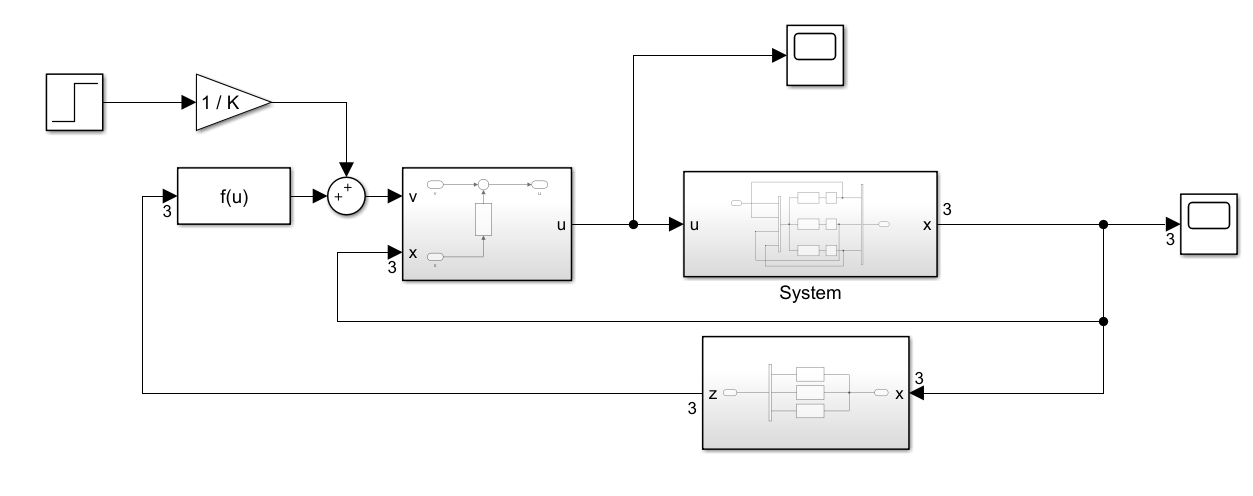
\includegraphics[width=0.8\linewidth]{ModelRiadenia}
		\caption{Bloková schéma systému s nelineárnym riadením}
		\label{fig:svlvs2_modelRiadenia}
	\end{figure}

	\begin{figure}[h!]
		\centering
		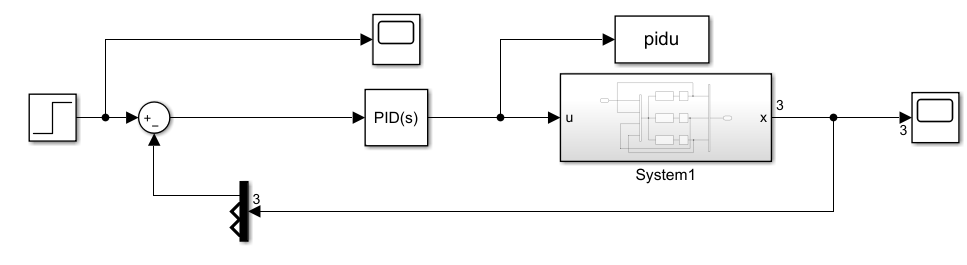
\includegraphics[width=0.8\linewidth]{ModelRiadeniaPID}
		\caption{Bloková schéma systému s PID regulátorom}
		\label{fig:svlvs2_modelRiadeniaPID}
	\end{figure}

Na \cref{fig:svlvs2_SimulaciaPID} môžeme vidieť, že takto navrhnutý PID regulátor dokáže pri malom skoku uriadiť náš systém. Pri väčšom skoku (\cref{fig:svlvs2_SimulaciaPIDVelkySkok}) sa náš uzavretý systém stal nestabilným. Je to spôsobené tým, že pri väčšej vzdialenosti od pracovného bodu sa chyba spôsobená linearizáciou zväčšuje a systému má iné vlastnosti ako systém, pre ktorý sme daný regulátor navrhovali.

Na \cref{fig:svlvs2_simulaciaNelin} a \cref{fig:svlvs2_simulaciaNelinU} je vidieť, že nelineárny regulátor dokázal uriadiť náš systém bez problémov aj na hodnotu 10.
	\begin{figure}[h!]
		\centering
		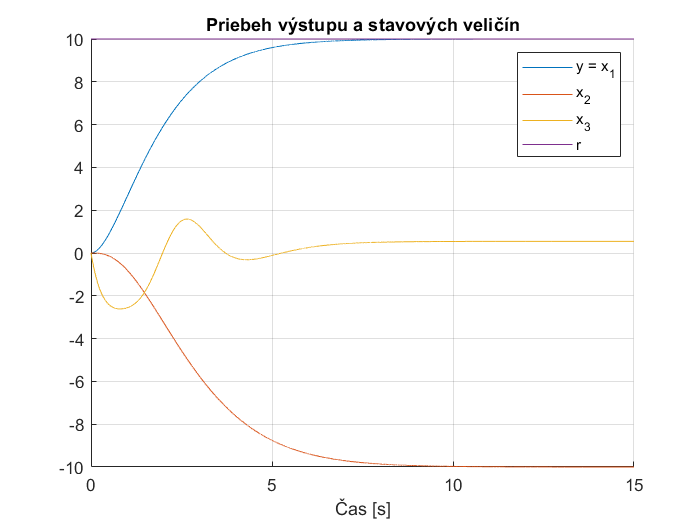
\includegraphics[width=0.8\linewidth]{SimulaciaNelin}
		\caption{Priebeh výstupu a stavových veličín s nelineárnym riadením}
		\label{fig:svlvs2_simulaciaNelin}
	\end{figure}

	\begin{figure}[h!]
		\centering
		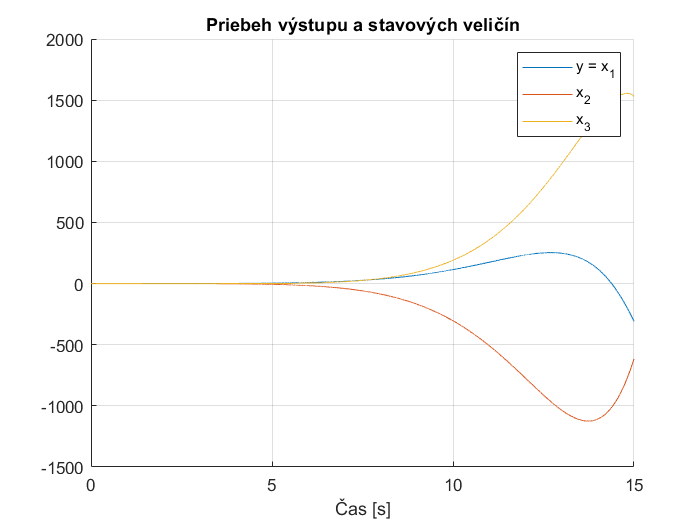
\includegraphics[width=0.8\linewidth]{SimulaciaPID}
		\caption{Priebeh výstupu a stavových veličín s PID (skok na 0.1)}
		\label{fig:svlvs2_SimulaciaPID}
	\end{figure}

	\begin{figure}[h!]
		\centering
		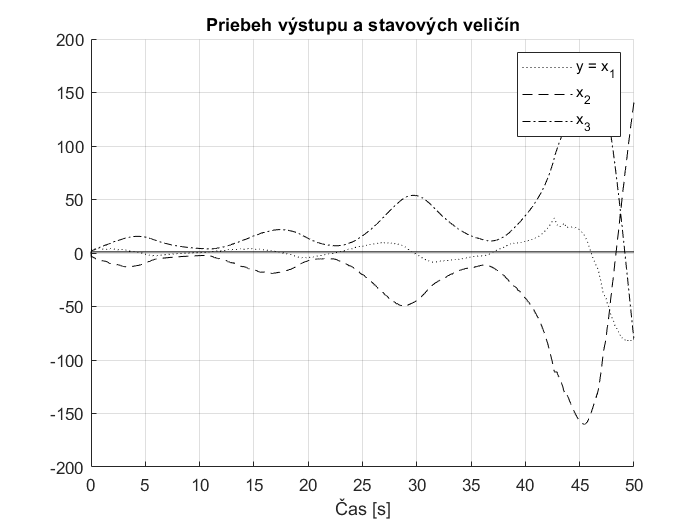
\includegraphics[width=0.8\linewidth]{SimulaciaPIDVelkySkok}
		\caption{Priebeh výstupu a stavových veličín s PID (skok na 1)}
		\label{fig:svlvs2_SimulaciaPIDVelkySkok}
	\end{figure}

	\begin{figure}[h!]
		\centering
		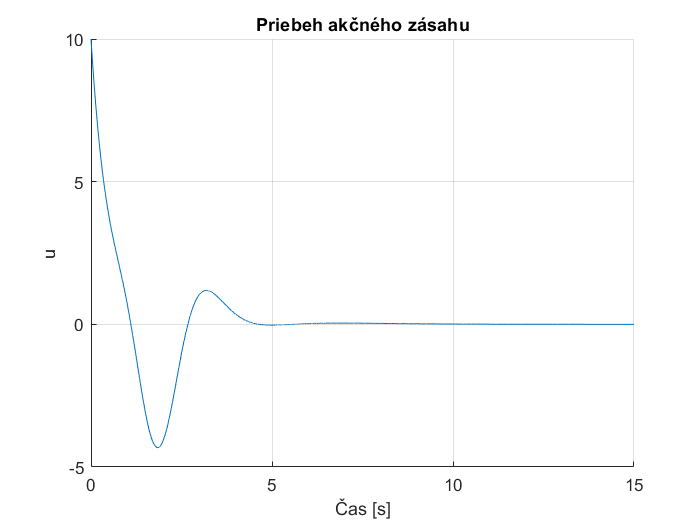
\includegraphics[width=0.8\linewidth]{SimulaciaNelinU}
		\caption{Priebeh akčného zásahu s nelineárnym riadením}
		\label{fig:svlvs2_simulaciaNelinU}
	\end{figure}

\end{document}
